\subsection{Vokabular}
\begin{frame}{Vokabular}
    \begin{itemize}
        \item<1-> Füllwörter: und, oder, im, in, \dots
        \item[$\Rightarrow$]<2-> Beschränkung des Vokabulars sinnvoll
    \end{itemize}

    \uncover<4->{
    \textbf{Idee}:
    \begin{itemize}
        \item<5-> Zufällige Beispielmenge von Texten für Vokabularbildung betrachten
        \item<6-> Gini-Koeffizient nutzen
    \end{itemize}
    }
\end{frame}

\begin{frame}{Gini-Koeffizient}
    \begin{itemize}
        \item<1-> statistisches Maß für Ungleichverteilung
        \item<2-> $g = \sum_i p_i^2$ mit $p_i$ als relative Häufigkeit
        \item<3-> $g \in (0, 1]$
        \item<4-> $g$ nahe bei $1$ $\Rightarrow$ Wort ist stark ungleich verteilt
        \item[$\Rightarrow$]<5-> Nehme Top-$m$ Wörter mit höchstem
                  Gini-Koeffizient
    \end{itemize}
\end{frame}

\begin{frame}{Gini-Koeffizient}
    \begin{center}
        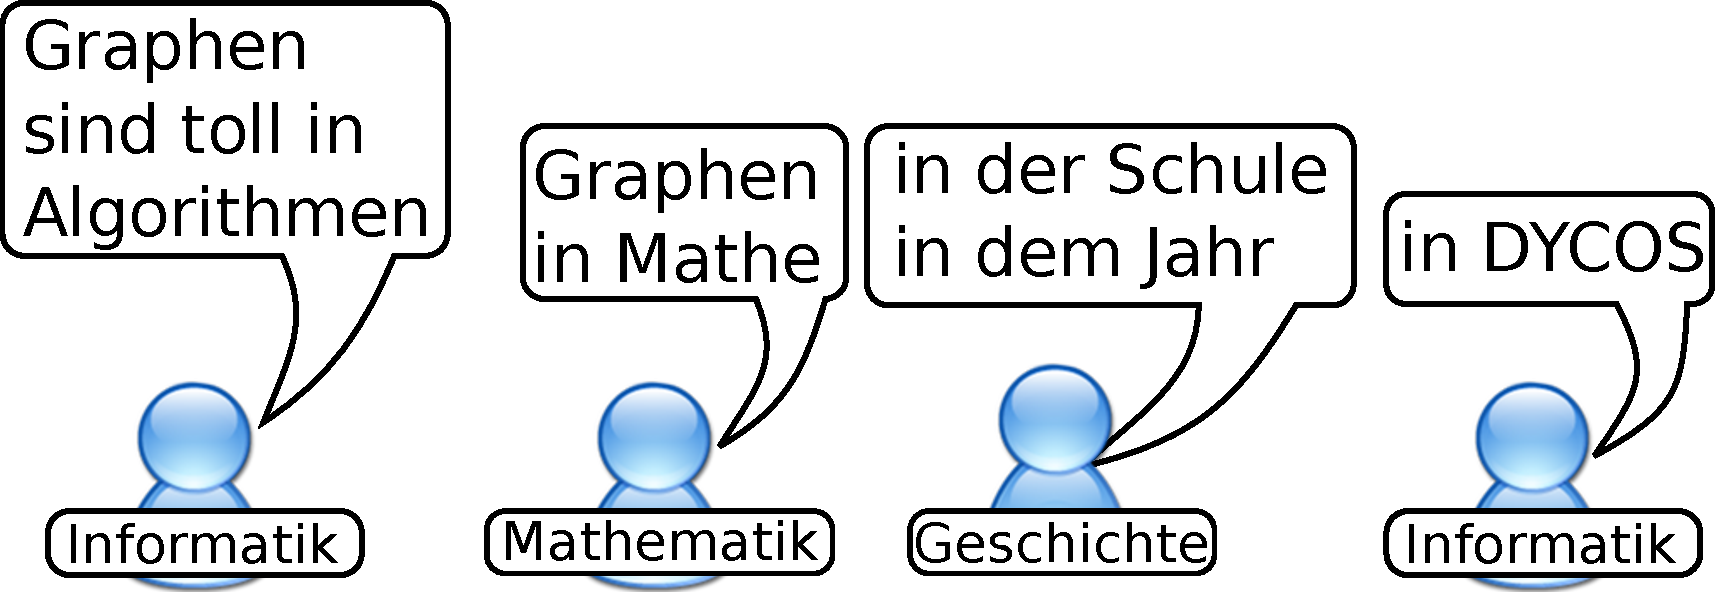
\includegraphics[width=\textwidth,height=0.4\textheight,keepaspectratio]{../images/gini-example.pdf}
    \end{center}

    \uncover<2->{Beispiel: \enquote{in}}
    \begin{itemize}
        \item<3-> Vorkommen insgesamt: $5 \times$
        \item<4-> Vorkommen in \enquote{Informatik} $2\times \Rightarrow p_1 = \frac{2}{5}$
        \item<5-> Vorkommen in \enquote{Mathematik} $1\times \Rightarrow p_2 = \frac{1}{5}$
        \item<6-> Vorkommen in \enquote{Geschichte} $2\times \Rightarrow p_2 = \frac{2}{5}$
        \item<7-> Gini-Koeffizient: $\left (\frac{2}{5} \right )^2 + \left (\frac{1}{5} \right )^2 + \left (\frac{2}{5} \right )^2 = \frac{9}{25}$
    \end{itemize}
\end{frame}
